%%%%%%%%%%%%%%%%%%%%%%%%%
\section{State of the Art} \label{stateOfTheArt}
%%%%%%%%%%%%%%%%%%%%%%%%%
City visualization is a subject undergoing intense study, therefore it is easy to find new projects about it everyday on the Internet. Still, the uniqueness of \applicationName\ resides on the fact that it provides not only a visualization of a city but, above all, it gives the user the possibility to interact with the city itself through a simple system of visual queries.\\

Before getting into the details with \applicationName, we will clarify the current state of city visualization and, since the projects about this topic are so various and so many, in this Chapter, we will present the ones that relate most with the final outcome of this Bachelor Project.\\

At first, we will present some 3D--city--model based on OpenStreetMap data, as {\bf OSMBuildings}, {\bf F4 Map} and {\bf ViziCities}. Then, we will introduce the {\bf Cesium framework}, since it has been used as a basis for \applicationName. At the end, we will analyze the work done by the {\bf Swiss Geospatial Portal} (still using Cesium), in order to compare it with the application described in this report. 
\subsection{OpenStreetMap--Based Frameworks}
OpenStreetMap\footnote{OpenStreetMap: phttp://www.openstreetmap.org/} is a project that creates and distributes free geographic data for the world. During the last decade, the third dimension has become a growing topic at OpenStreetMap, so it is now possible to add detailed buildings and a lot of minor objects. Here, some of the frameworks that use this data, will be analyzed.
\subsubsection{OSMBuildings}
OSMBuildings\footnote{OSMBuildings: https://osmbuildings.org/} is an engine for displaying 3D buildings on a web map. It uses information on buildings provided by OpenStreetMap and it renders them on a map layer.\\ Although in some cases, buildings are very detailed (e.g., in big cities like New York or Berlin), it provides only a visualization without any kind of interaction.
\begin{figure} [H]
\centering
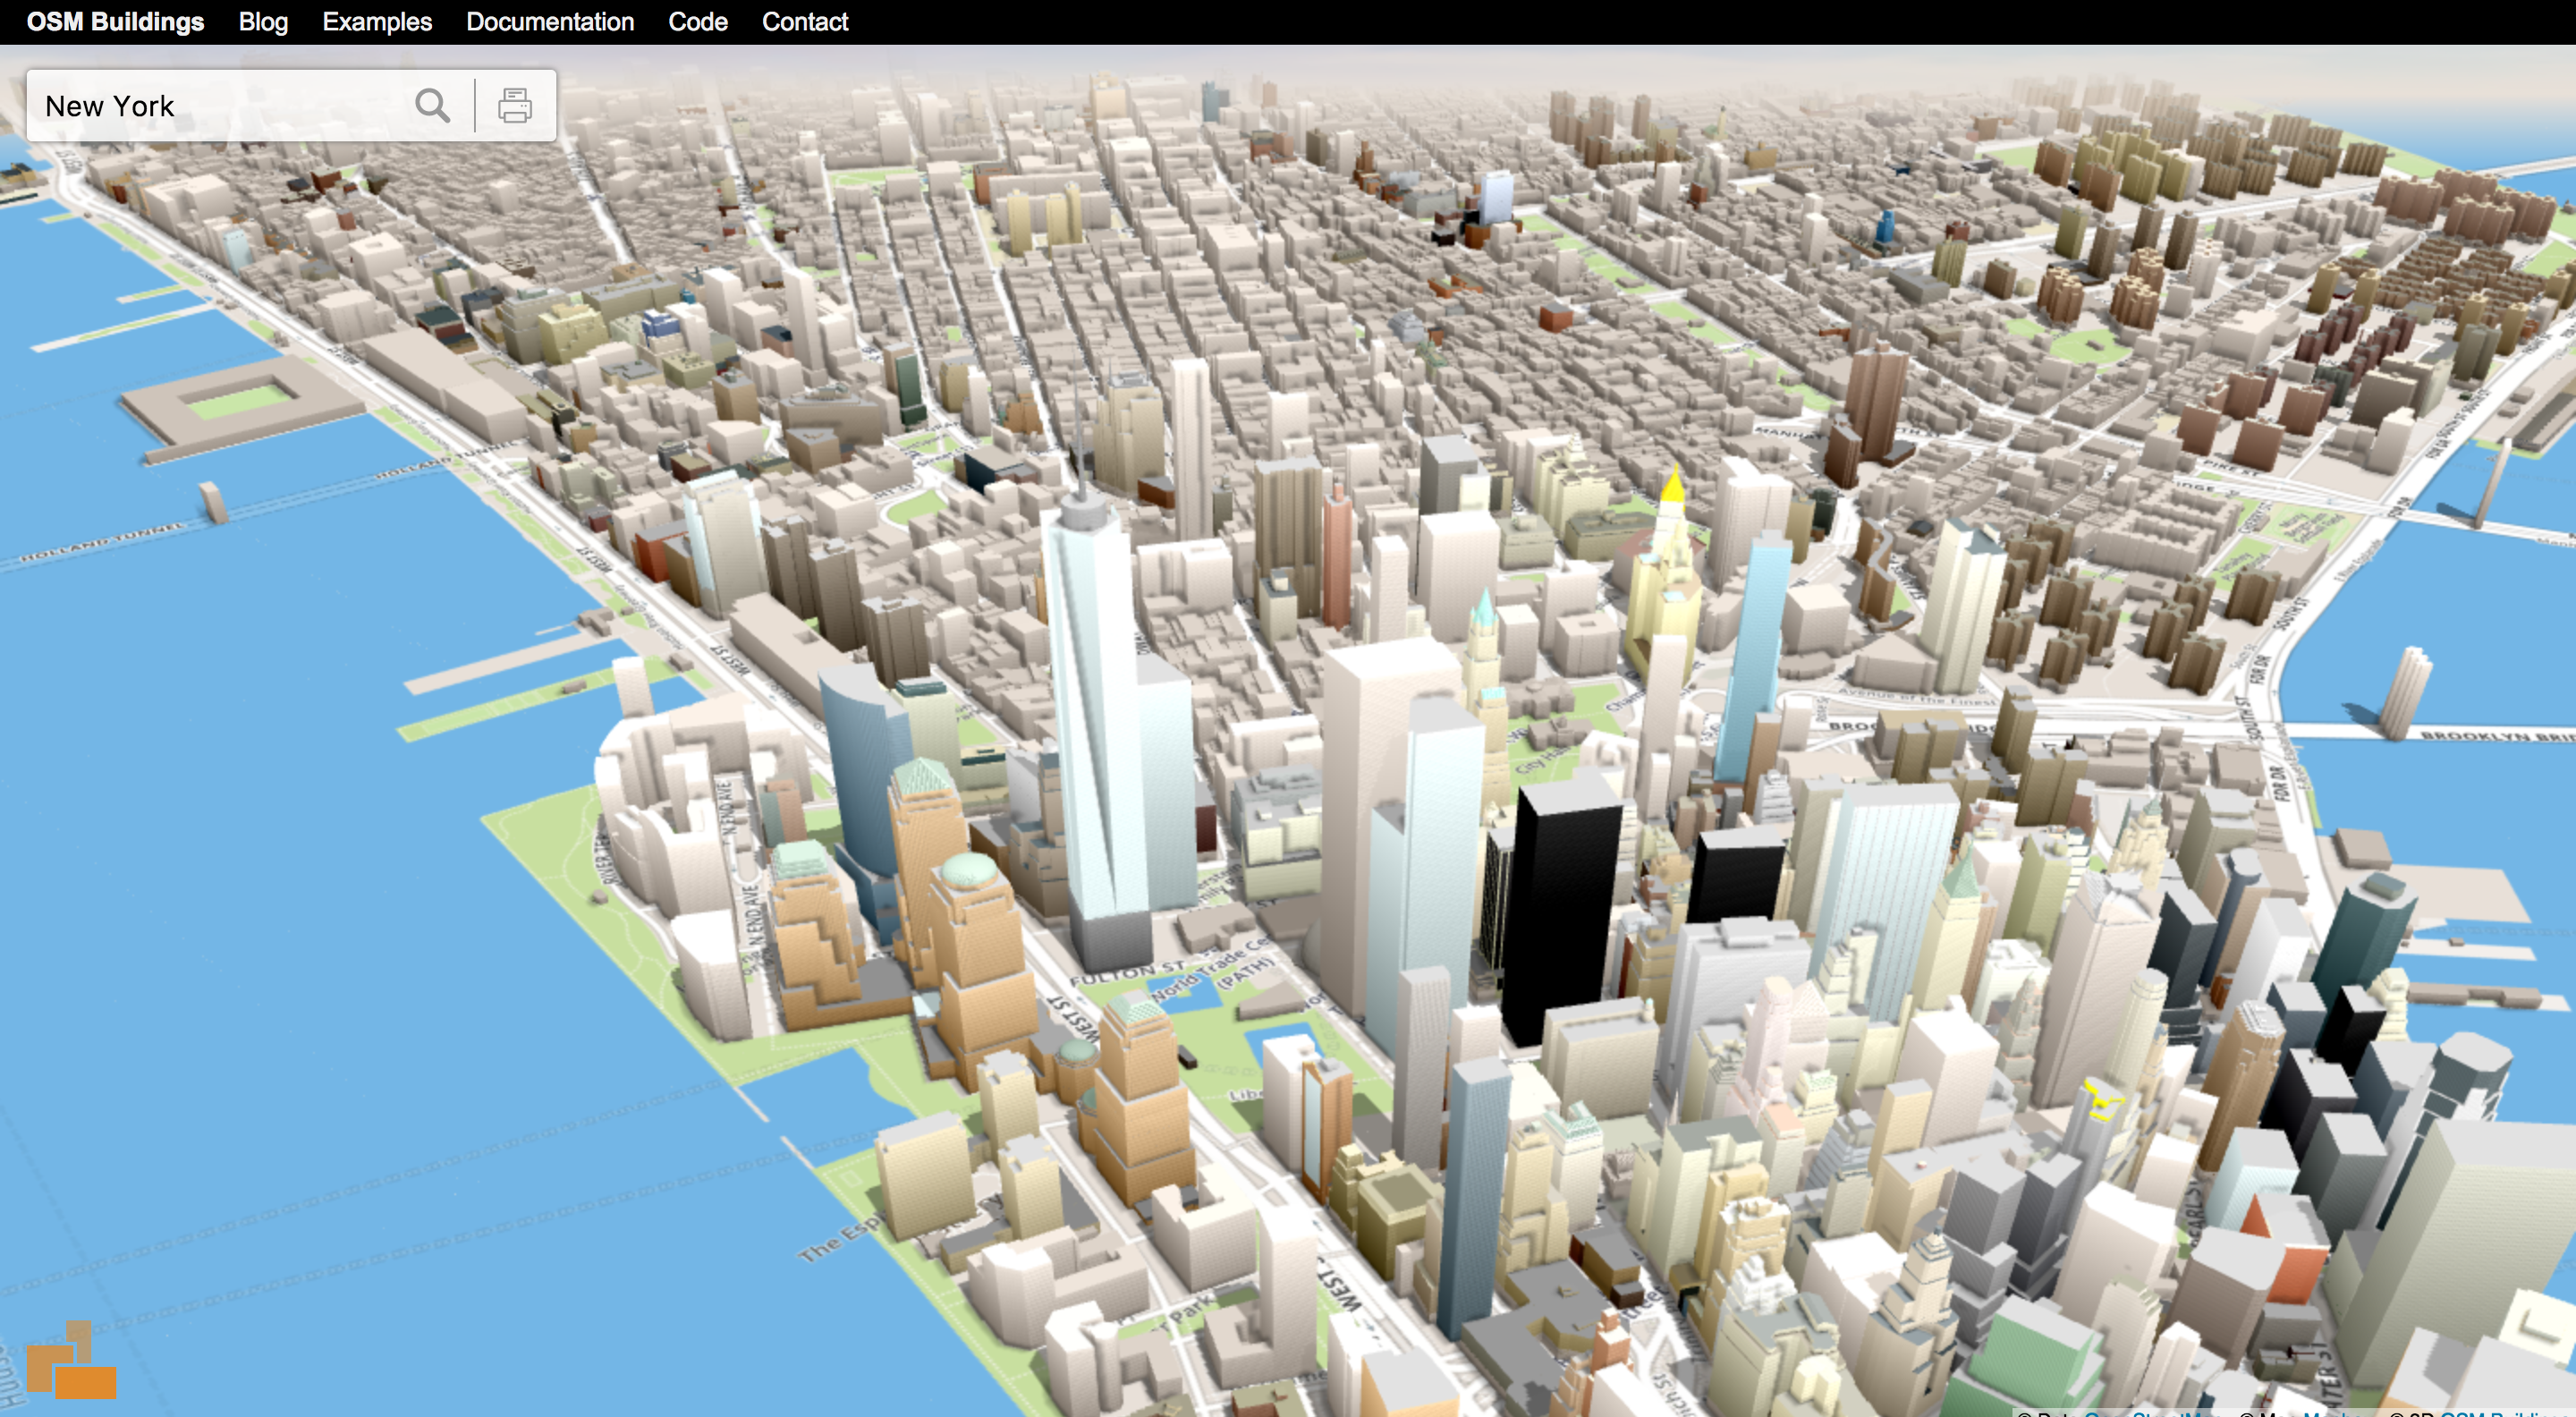
\includegraphics[width=0.8\textwidth]{chapter2/images/OSM_Building}
\caption{A visualization of New York city using OSMBuildings}
\label{fig:OSM_Building}
\end{figure}

\subsubsection{F4 Map}
The F4 Map\footnote{F4 Map: http://demo.f4map.com/} is an OSM-based 3D map using the WebGL technology. Also, this map uses Open Street Map's buildings but also adds some non--OSM--provided features like trees, cranes and other data.\\
 F4 Map uses 3D models of some specific buildings that are not based on buildings data in OpenStreetMap (e.g. the Eiffel Tower in the example below).
\begin{figure}[H]
\centering
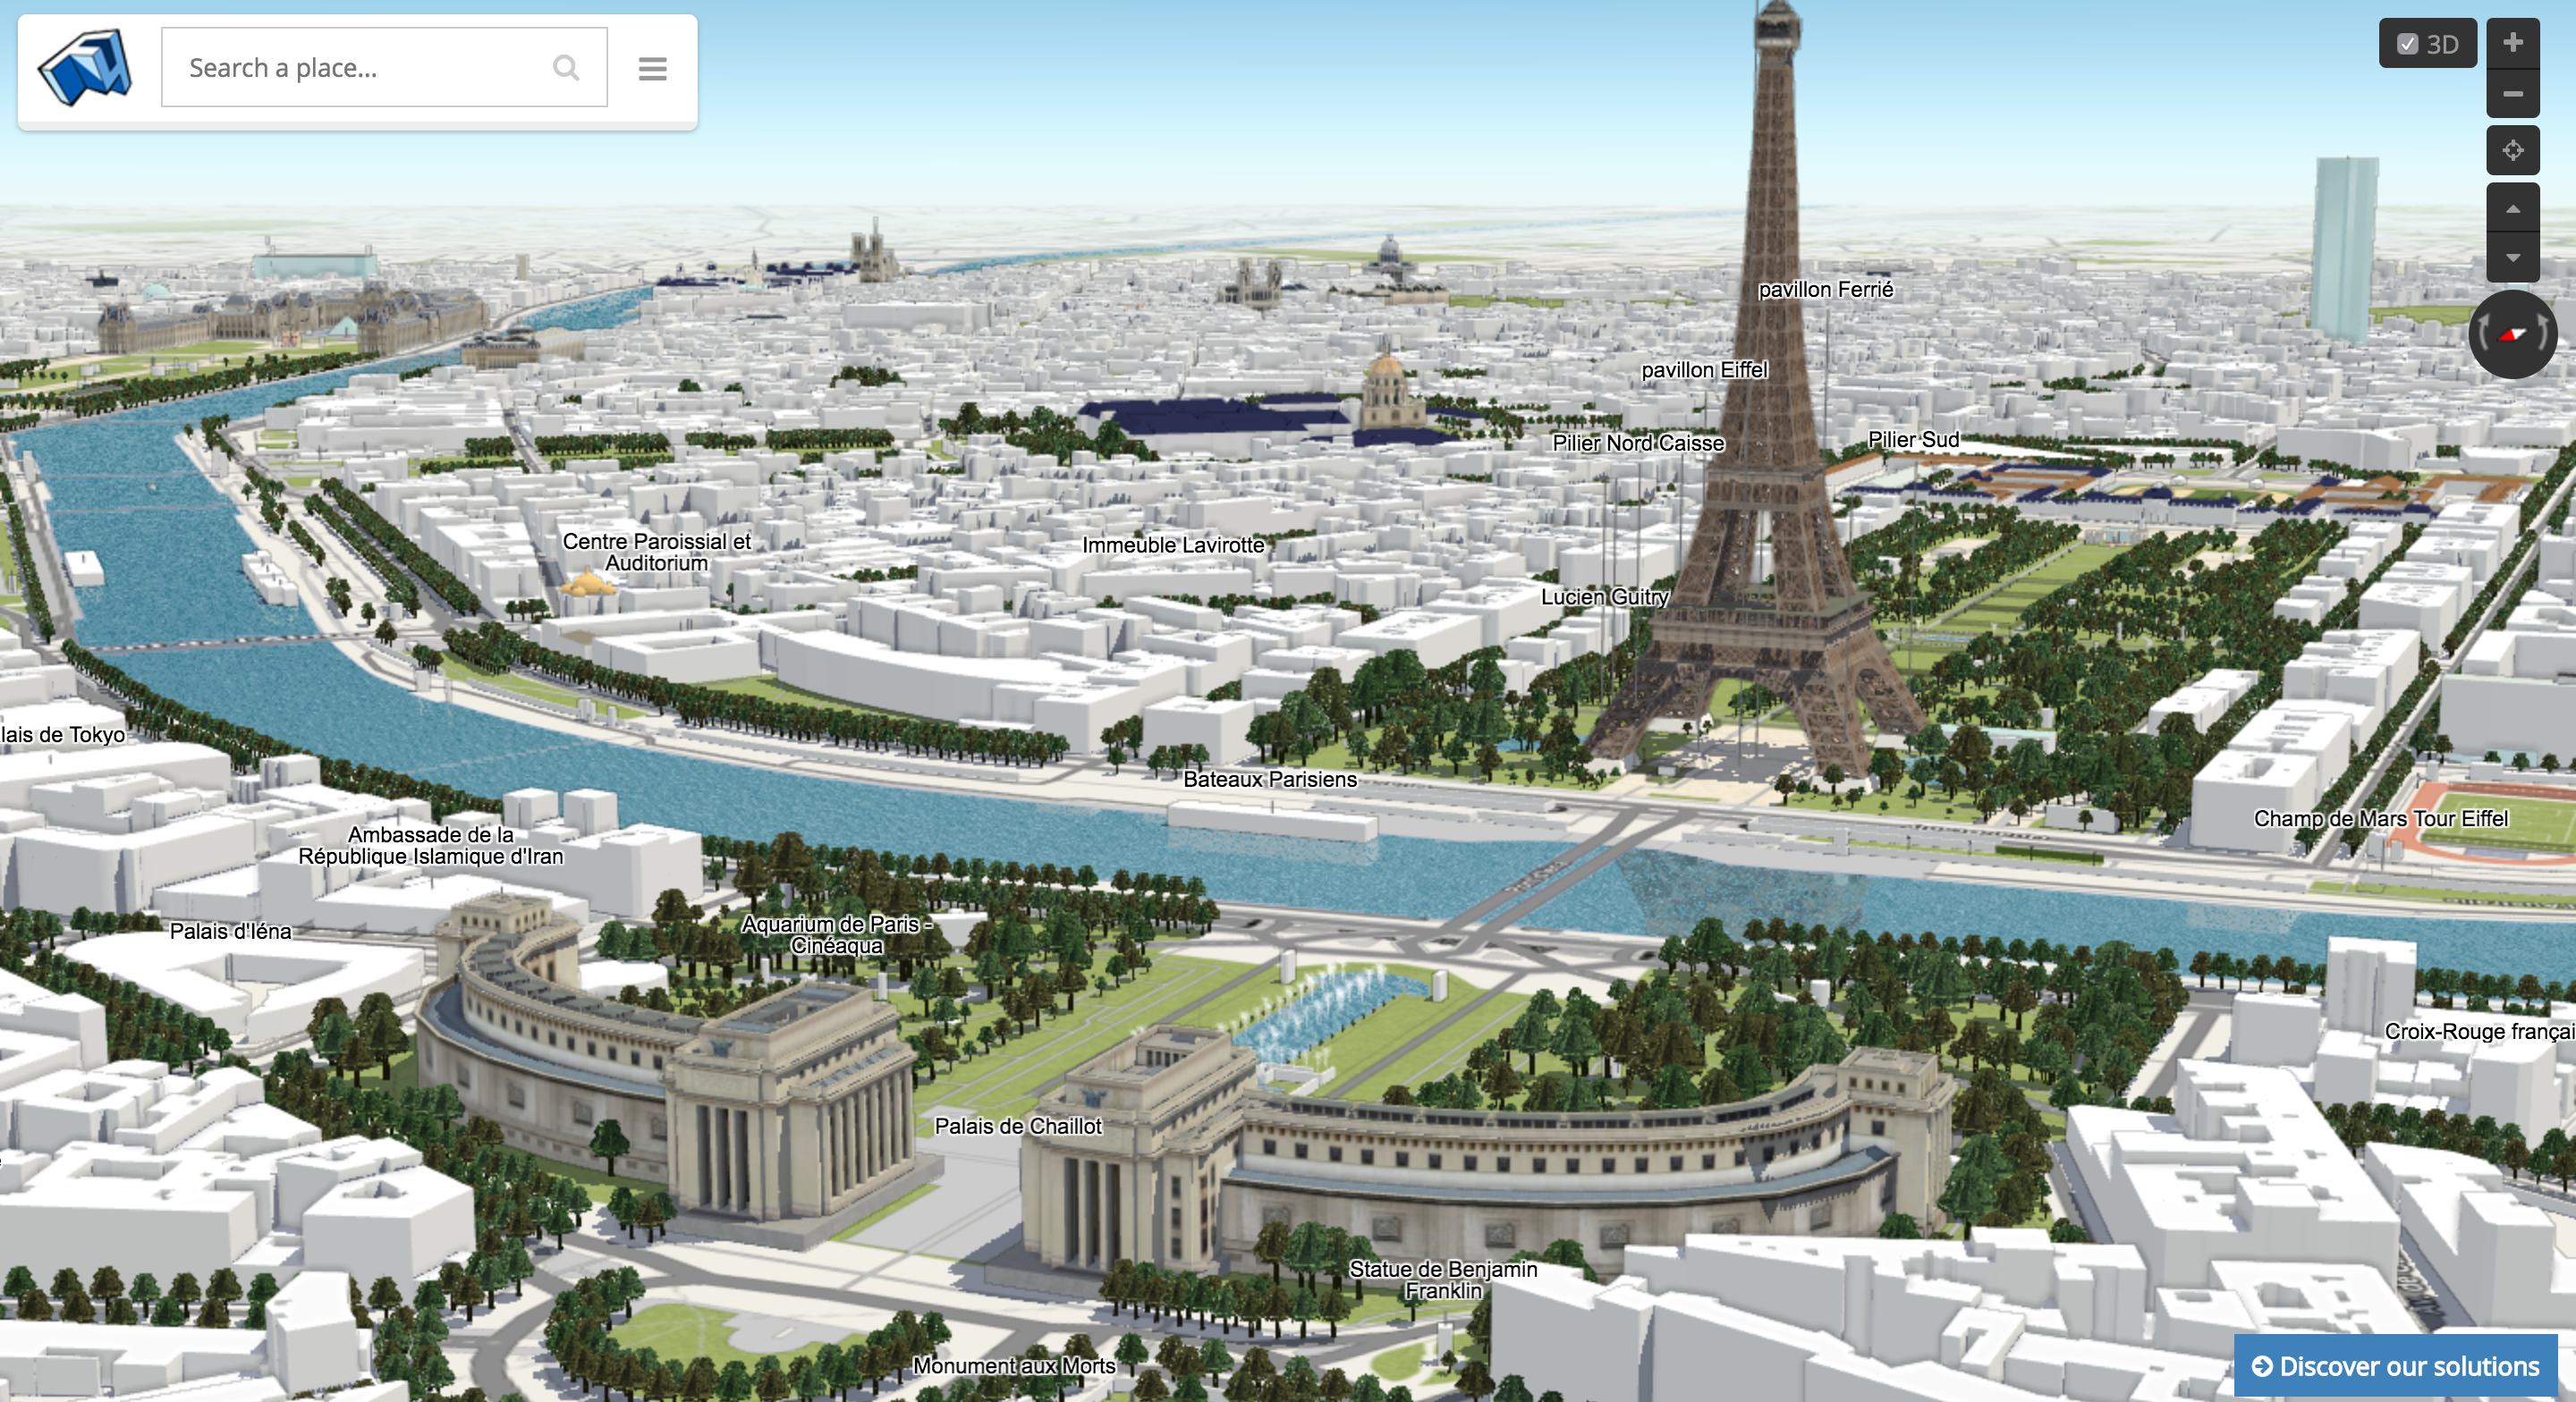
\includegraphics[width=0.8\textwidth]{chapter2/images/F4-Map}
\caption{A visualization of Paris using F4 Map}
\label{fig:F4-Map}
\end{figure}
Unfortunately, the F4 group does not provide any kind of documentation and this project is not open source.
\subsubsection{ViziCities}
The third and last map that uses OSM information about buildings is ViziCities\footnote{ViziCities: https://github.com/UDST/vizicities}, a framework for 3D geospatial visualization in the browser. Its code is available on GitHub since it is an OpenSource project but they are still at a prototypical version of what the application is intended to be.\\It allows the developer to add some useful information to the map like routes and GeoJSON (i.e., a format for encoding a variety of geographic data structures) but is still very limited and not very prone to interactivity. For example, use cases are accessible by different urls and they limit the user experience to just a visualization of buildings or roads. Therefore, it is not possible to interact with the entities shown in the city. 
\begin{figure}[H]
\centering
\includegraphics[width=0.8\textwidth]{chapter2/images/vizicities-Map}
\caption{A visualization of New York city using ViziCities}
\label{fig:vizicities-Map}
\end{figure}

\subsection{Cesium}
\begin{figure} [H]
\centering
\includegraphics[width=0.8\textwidth]{chapter2/images/cesium_logo}
\caption{Cesium logo and Cesium Virtual Globe}
\label{fig:cesium_logo}
\end{figure}
Cesium\footnote{Cesium: https://cesiumjs.org/} is an open-source JavaScript library for world-class 3D globes and maps that is used to create a web-based globe and map for visualizing dynamic data. This framework runs using WebGL, a JavaScript API for rendering 3D graphics within any compatible web browser that allows GPU--accelerated usage of physics, image processing, and effects as part of the web page canvas.\\ 
The features that Cesium provides are the following:
\begin{itemize}
	\item {\bf A virtual globe:} a three-dimensional software model or representation of the Earth that allows the user to freely move around in the virtual environment by changing the viewing angle and position.
	\item {\bf Different imagery providers:} it allows drawing and layerering on high-resolution imagery (maps) from several standard services directly on the virtual globe. Between these services there are Bing\footnote{Bing Imagery Provider: https://www.bing.com/maps} and MapBox\footnote{MapBox Imagery Provider: https://www.mapbox.com/} as shown in Figure \ref{fig:Bing_Mapbox-Map}.
	\begin{figure} [h]
		\centering
		\begin{subfigure}[b]{0.3\textwidth}
			\includegraphics[width=1\textwidth]{chapter2/images/Bing-Map}
			\caption{High-resolution, mesh-based terrain provided by Bing}
			\label{fig:Bing-Map}
		\end{subfigure}
		 \qquad
		\begin{subfigure}[b]{0.3\textwidth}
			\includegraphics[width=0.993\textwidth]{chapter2/images/Mapbox-Map}
			\caption{Streets basic imagery provided by Mapbox}
			\label{fig:Mapbox-Map}
		\end{subfigure}
		\caption{Example of two imagery providers available on Cesium}
		\label{fig:Bing_Mapbox-Map}
	\end{figure}

	\item {\bf Different terrain providers:} it allows visualizing global high-resolution terrains and water effects for oceans, lakes, and rivers, but mainly the possibility to represent mountain peaks, valleys, and other terrain features. A service that provides these terrains is STK\footnote{STK Terrain Provider: https://cesiumjs.org/data-and-assets/terrain/stk-world-terrain.html}. Figure \ref{fig:2D_3D-Map} compares the standard Cesium terrain which uses the standard WGS84 Ellipsoid\footnote{WGS84 Standard: http://wiki.gis.com/wiki/index.php/WGS84} (i.e., with no elevation) with the one provided by STK.
	\begin{figure} [H]
		\centering
		\begin{subfigure}[b]{0.3\textwidth}
			\includegraphics[width=1\textwidth]{chapter2/images/2D-Map}
			\caption{The standard WGS84 Ellipsoid}
			\label{fig:2D-Map}
		\end{subfigure}
		 \qquad
		\begin{subfigure}[b]{0.3\textwidth}
			\includegraphics[width=0.993\textwidth]{chapter2/images/3D-Map}
			\caption{Terrain meshes provided by STK}
			\label{fig:3D-Map}
		\end{subfigure}
		\caption{Example of two terrain providers available on Cesium, this shows the benefits of a 3D globe compared to a 2D map.}
		\label{fig:2D_3D-Map}
	\end{figure}
	\item {\bf Huge number of APIs provided:} since the uses of Cesium are really various, Cesium provides a very high number of APIs to control every aspect of the web application, i.e., draw every kind of geometry, handle animations, etc\dots. The official website of Cesium also provides a complete documentation, various examples, and playgrounds.
\end{itemize} 
\subsubsection{Cesium: 3D-Tiles}
Cesium's repository on GitHub\footnote{Cesium GitHub Repository: https://github.com/AnalyticalGraphicsInc/cesium} has an open fork called ``3D-Tiles''\footnote{Cesium 3D-Tiles Fork: https://github.com/AnalyticalGraphicsInc/3d-tiles}. As specified by the contributors of this fork:  ``In 3D Tiles, a tileset is a set of tiles organized in a spatial data structure, the tree. Each tile has a bounding volume completely enclosing its contents. The tree has spatial coherence; the content for child tiles are completely inside the parent's bounding volume. To allow flexibility, the tree can be any spatial data structure with spatial coherence, including k-d trees, quadtrees, octrees, and grids.''
\begin{figure} [H]
\centering
\includegraphics[width=0.8\textwidth]{chapter2/images/NewYorkCityCesium3dTiles}
\caption{An example showing a 3D visualization of the city of New York. Using Cesium 3D Tiles Technology}
\label{fig:NewYorkCityCesium3dTiles}
\end{figure}
Unfortunately, being Cesium 3D--Tiles still under development, no public documentation has been provided. Still, in a recent post on Cesium Forum, one of the main Cesium--developers stated that Cesium 3D--tiles fork will be soon merged to the main branch and therefore a complete documentation will be provided as well. \\In the meantime, Cesium 3D--Tiles developers are available to help programmers interested in using this technology using their forum\footnote{Developers' help forum: http://tiny.cc/884tly}.

\subsubsection{Swiss Geospatial Portal Using 3D Tiles}
Swisstopo\footnote{Swisstopo: https://www.swisstopo.admin.ch/it/home.html} , the Swiss Federal Geoportal, is a federal government platform that facilitates public access to Swiss spatial data.
This agency produces detailed maps of Switzerland and also documents geological, geodesic(i.e., a service that denotes the shortest possible line between two points on the Earth), and topographical changes in the landscape.\\
Swisstopo is one of the pioneers in implementing 3D Tiles to process its extensive data collection and Cesium to visualize it. The beta visualization of their 3D Geoportal is available, it makes their national geodata collection widely available\footnote{Swisstopo implementing 3D--Tiles: http://tiny.cc/0s5tly}.
\begin{figure} [H]
\centering
\includegraphics[width=0.8\textwidth]{chapter2/images/BernCitySwissTopo}
\caption{A 3D visualization of the city of Bern in the Swiss Geospatial Portal. Using Cesium 3D Tiles Technology}
\label{fig:BernCitySwissTopo}
\end{figure}
The work done by Swisstopo, so far, consists in placing the 3D--models of buildings in some of the cities in the norther part of Switzerland (e.g., Bern, Rapperswil-Jona, Winterthur, etc\dots ). It is not provided any kind of interaction with the buildings. Also, the city of Lugano (used as a test case of visualization for this project), is not currently available in the 3D--visualization provided by Swisstopo.\\
Swisstopo provides a service in which it is possible to buy the 3D--models of the buildings, they are not highly detailed but they contain important information about the shape of the roof as can be seen in Figure\ref{fig:swisstopoBuildingModel}.
\begin{figure} [H]
\centering
\includegraphics[width=0.5\textwidth]{chapter2/images/swisstopoBuildingModel}
\caption{A 3D--Model of a building provided by the Swiss Geospatial Portal and used in 3D--Tiles}
\label{fig:swisstopoBuildingModel}
\end{figure}
For this reason, during the last period of the development of \applicationName, models of the city of Lugano have been bought. The use of these models may be done as one of the future developments of this application. This will be discussed at the end of this report.